\section{Grouping and Events}
\label{grouping}
\ifxHPTDC{
    If \textsf{config.tdc\tu mode} is set to \textsf{\PREFIX TDC\tu MODE\tu CONTINOUS} the TDC will operate in grouping mode. 
    This setting only affects data collected using the \textsf{\prefix Read()} method. Data collected using \textsf{\prefix ReadHits()} will always be continous. 
}{} 

In typical applications a start hit is followed by a manifold of hits on e.g. a detector. 
The hits recorded are managed in groups (which are called ``events'' in some applications). 
Figure \ref{fig:grouping} shows a corresponding timing diagram. The user can define the range of a group, i.e. the time window within which hits 
on the stop channels are recorded, in software. Hits occurring outside of that time window are discarded. 
 Different ranges can be set for each of the 4 stop channels by setting corresponding configuration.channel[n].start and .stop values in the channel configuration. 

 \ifxHPTDC{
     The values are configured in picoseconds. Negative values can be used in common stop applications.
     \[ -2^{31} <= start <= stop <= 2^{31}-1 \]
 }{
    The values need to be set as multiples of the bin size and must not be negative.
    \[ 0 <= start <= stop <= 2^{16}-1 \]
 }


%
\begin{figure*}[ht]
    \begin{center}
        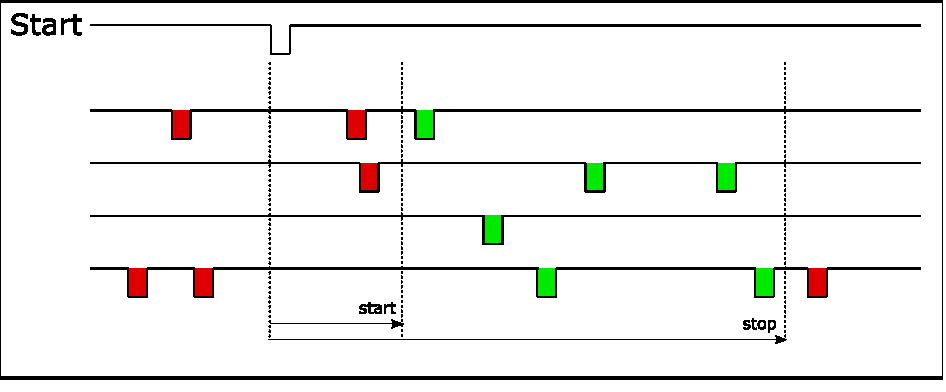
\includegraphics[width=0.7\textwidth]{figures/grouping.pdf}
        \caption{Acquired hits are merged to groups as explained in the text.\label{fig:grouping}}
    \end{center}
\end{figure*}


%